\chapter*{\FontH{\Huge Der grosse Clown kann fliegen}}
\addcontentsline{toc}{chapter}{Der grosse Clown kann fliegen}
\lettrine[lines=3]{\color{red}L}{ouis} und seine Eltern kommen gerade vom Stadtfest zurück. Er hatte im Karussell fahren dürfen und hatte einen Schleckstengel bekommen, der viel grösser ist als seine Hand. Aber sein ganzer Stolz gehört einem Luftballon, der aussieht wie das Gesicht eines Clowns. Rote Nase, rote Lippen mit weissem Rand, genau wie bei den Augen und dazu gelbe Haare. Louis hält den Ballon auf dem Arm.

Gerade als Mama die Tür aufschliesst, kommt die Nachbarin Frau Schweizer. Auch sie hat die Lippen so rot geschminkt wie der Clown, aber der weisse Rand fehlt. Dafür hat sie furchtbar lange Fingernägel auf die immer wechselnd Muster gemalt sind. Louis hat immer ein bisschen Angst vor diesen Fingernägeln und muss sie immer ansehen, weswegen Frau Schweizer ihn für besonders schüchtern hält.

\enquote{Hach Frau Reichenbach}, ruft sie, \enquote{Sie können es nicht glauben. Meine Neffin liegt im Krankenhaus, ein Unfall, wissen Sie. Die sollte ich dringend besuchen. Ob sie nicht so lange auf Leika aufpassen könnten? Heute Abend bin ich bestimmt zurück.} Seltsamerweise redet Frau Schweizer immer nur mit Mama und nie mit Papa, denkt Louis, vielleicht weil der aus einem anderen Land kommt und nicht so gut Deutsch kann.

Leika ist der Hund von Frau Schweizer. Ein sehr kleiner weisser Hund, der immer kläfft. Louis kann Leika deswegen nicht besonders leiden. Nie kann er mit dem Ball draussen spielen, wenn Leika in der Nähe ist. Der Hund springt dann immer hinter dem Ball her und versuchte den zu beissen, was aber nie klappt, denn sein Maul ist viel zu klein. Frau Schweizer ruft dann immer, dass Leika doch nur spielen will, womit Louis aber auch nicht geholfen ist. Gegen den Ball treten geht dann nicht mehr. Frau Schweizer hat das aber noch nie gestört.

Aber einen Nachmittag lang kann ja nicht so schlimm sein, denkt sich Louis. Was für ein Irrtum! Schon als allererstes schnappt sich Leika den linken Hausschuh von Louis und rennt damit auf den Balkon.

\enquote{Zieh endlich deine Hausschuhe an!} hört Louis Papa rufen. Pff, als ob er das nicht vorgehabt hätte. Aber wie denn ohne Schuhe? Dann schmeisst Leika den Turm um, den Louis und Papa heute Morgen, als Mama noch geschlafen hat, gebaut haben. Louis fängt an mit Leika zu schimpfen, aber Mama ruft aus der Küche, dass das doch nicht so schlimm sei und man den Turm neu bauen könne. Aber Louis will keinen neuen Turm, er will den Turm wieder haben und ist eingeschnappt. Wieso bekommt der Hund jetzt auch noch Recht! Ungerecht ist das. Er streckt Leika die Zunge raus und schiesst ein Kissen nach ihm.

\enquote{Jetzt reicht es aber!} Papa und Mama sind ärgerlich. Mit Kissen nach kleinen Hunden schiessen ist nicht in Ordnung, finden die. Als ob dem das weh tun könnte.
\begin{figure}[ht]
\centering
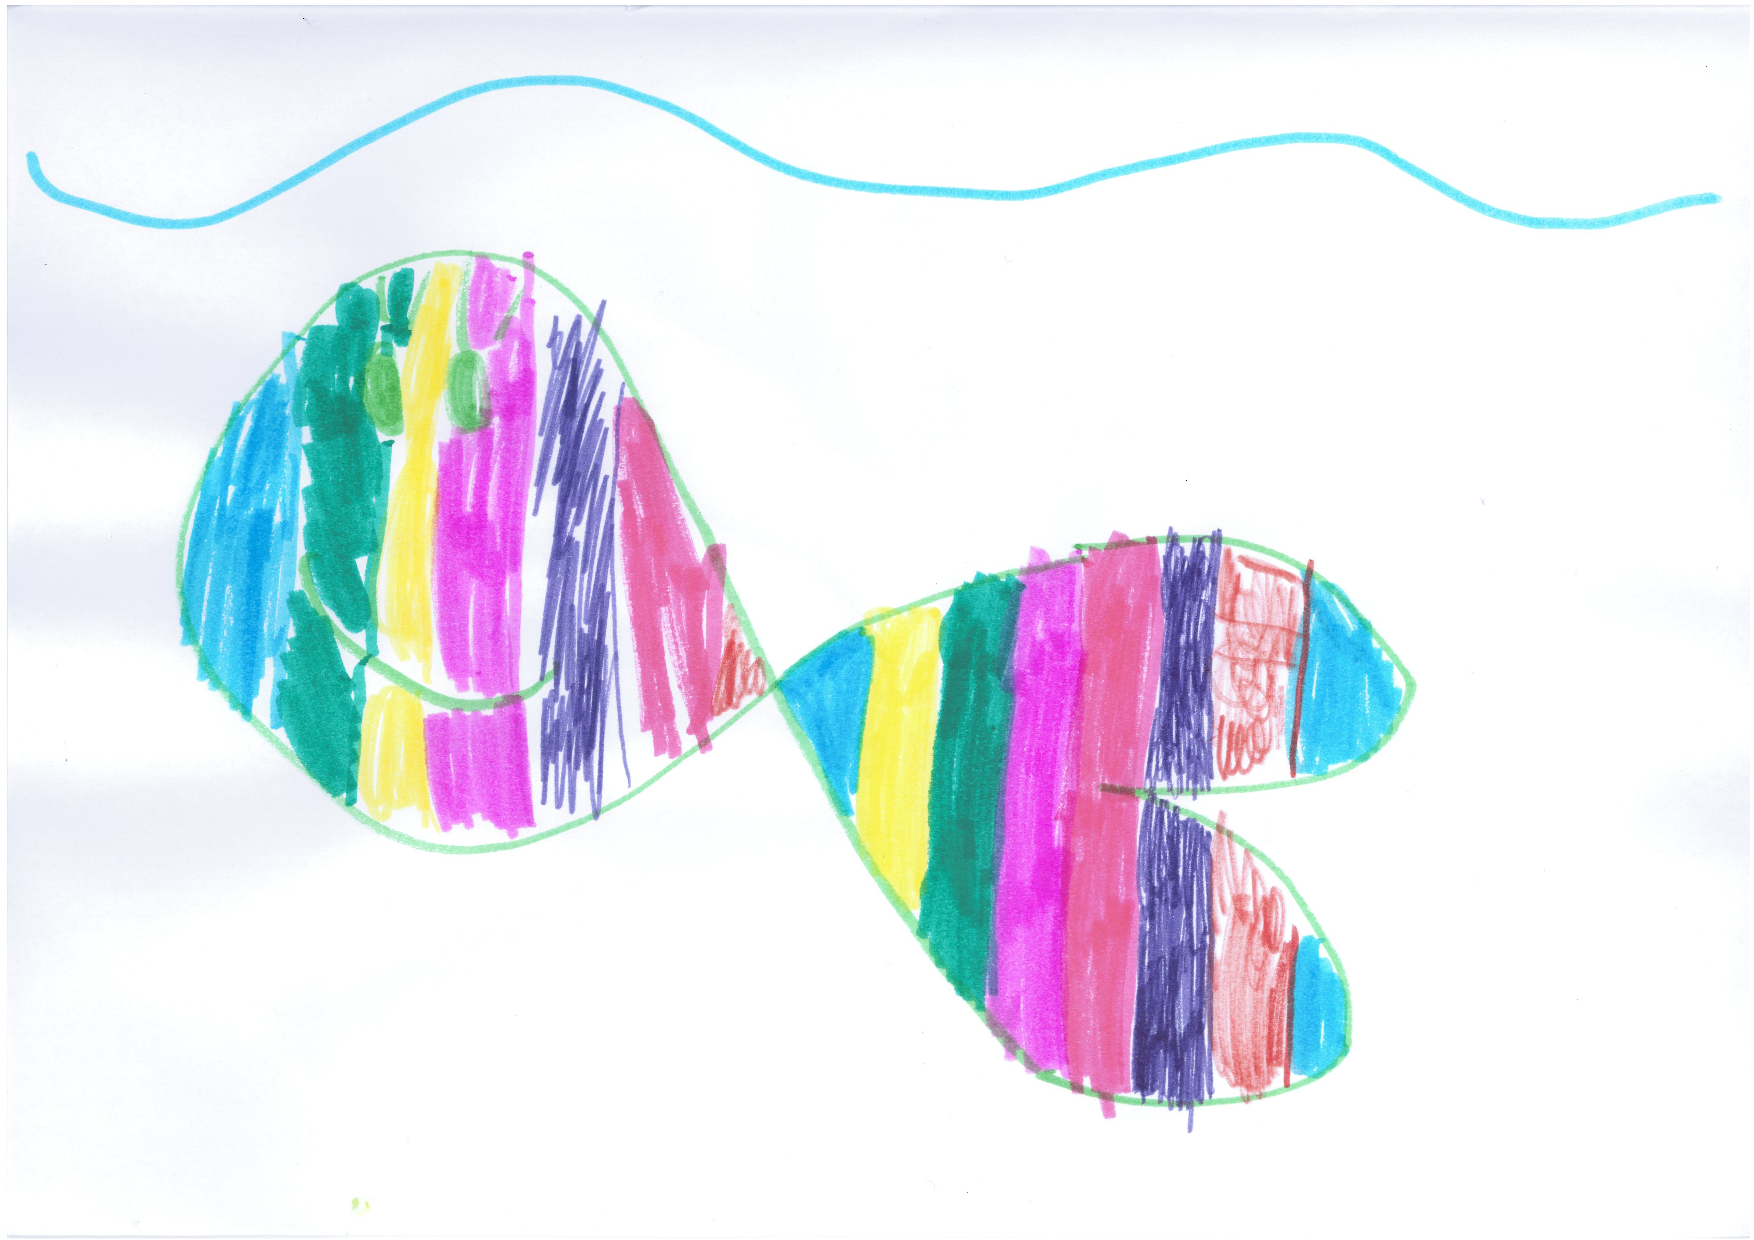
\includegraphics[width=\textwidth]{bilder/clown.pdf}
\end{figure}
\enquote{Und ab in dein Zimmer, Freundchen, bis es Mittag gibt!} heisst es dann auch noch. So eine Gemeinheit, aber egal, Louis will sowieso in sein Zimmer und etwas spielen. Tür zu und erst wieder raus kommen, wenn Frau Schweizer Leika abgeholt hat, so ist sein Plan. Aber bevor er die Tür schliessen kann, wird Leika auch in sein Zimmer geschoben. 

\enquote{Du spielst jetzt auch mit Leika}, sagt Mama, \enquote{Wir wollen hier noch im Wohnzimmer putzen und da stört ein Hund sehr. Spiel du mit ihm.}

Das hatte noch gefehlt! Jetzt muss sich Louis um Leika kümmern. Mist! Aber vielleicht genügt es ja, ihn zu ignorieren. Louis sieht sich gerade um, mit was er als erstes spielen soll, als Leika furchtbar zu bellen anfängt und sich auf den neuen Clowns-Ballon stürzt. Ausgerechnet! Gerade noch kann Louis ihn wegreissen. Das war knapp. Einen Ball kann Leika nicht zerbeissen, bei einem Ballon ist sich Louis da nicht so sicher.

Er hält den Clown so hoch er kann, aber Leika springt immer wieder an ihm hoch und versucht ihn zu schnappen. So ist der Clownsballon zwar erst einmal in Sicherheit, aber lange kann er die Arme nicht so nach oben halten. Dann eben in das Regal mit dem Ballon. Das erste Fach, bei dem es Louis probiert, ist schon voll. Kuscheltiere. Das zweite ist zu klein. Beim dritten klappt es. Triumphieren schiebt Louis den Ballon in das Fach.

Leika bekleitet Louis dabei durch ununterbrochenes Bellen, denn er will unbedingt an diesen Ballon kommen. So sind Hunde halt, das ist ihre Art zu spielen, aber es nervt eben doch. Plötzlich ist Leika mit einem Sprung auf dem Schreibtisch. Louis hätte nie gedacht, dass ein so kleiner Hund so hoch springen kann. Ein bisschen beeindruckt ist Louis schon. Aber er merkt sofort, was Leika vor hat. Vom Schreibtisch ist es nicht mehr weit bis zum Regalfach, aus dem der Clown lacht. 

Louis kann im letzten Moment den Clownsballon aus dem Regal reissen, legt ihn hinter sich und fängt an, mit Leika zu schimpfen. Wie genau das passieren konnte, weiss Louis später nicht mehr. Aber der Balkon fällt irgendwie aus dem offenen Fenster.

Selbst Leika verschlägt es den Atem. Louis und Leika sind still und sehen zum offenen Fenster und zu dem Ballon. Louis überlegt gerade, ob es wohl laut poltert, wenn so ein Clownsballon unten auf dem Boden aufschlägt. Und ob er dann wohl in tausend Scherben zerspringen wird, wie neulich Papas Glas, oder ob er nur eine grosse Beule bekommt, wie sein Spielzeugauto. Das wäre dann gar nicht so schlimm.

Aber es passiert etwas ganz anderes, etwas, womit weder Louis noch Leika gerechnet haben. Der Ballon fällt überhaupt nicht nach unten, sondern steigt in die Luft! Er sieht genau zu Louis und lacht ihn an. Der Wind drückt ihn nochmals gegen die Wand und dann steigt er immer höher, die Schnur, mit der ihn Louis gehalten hat, zieht er hinter sich her.

\begin{figure}[ht]
\centering
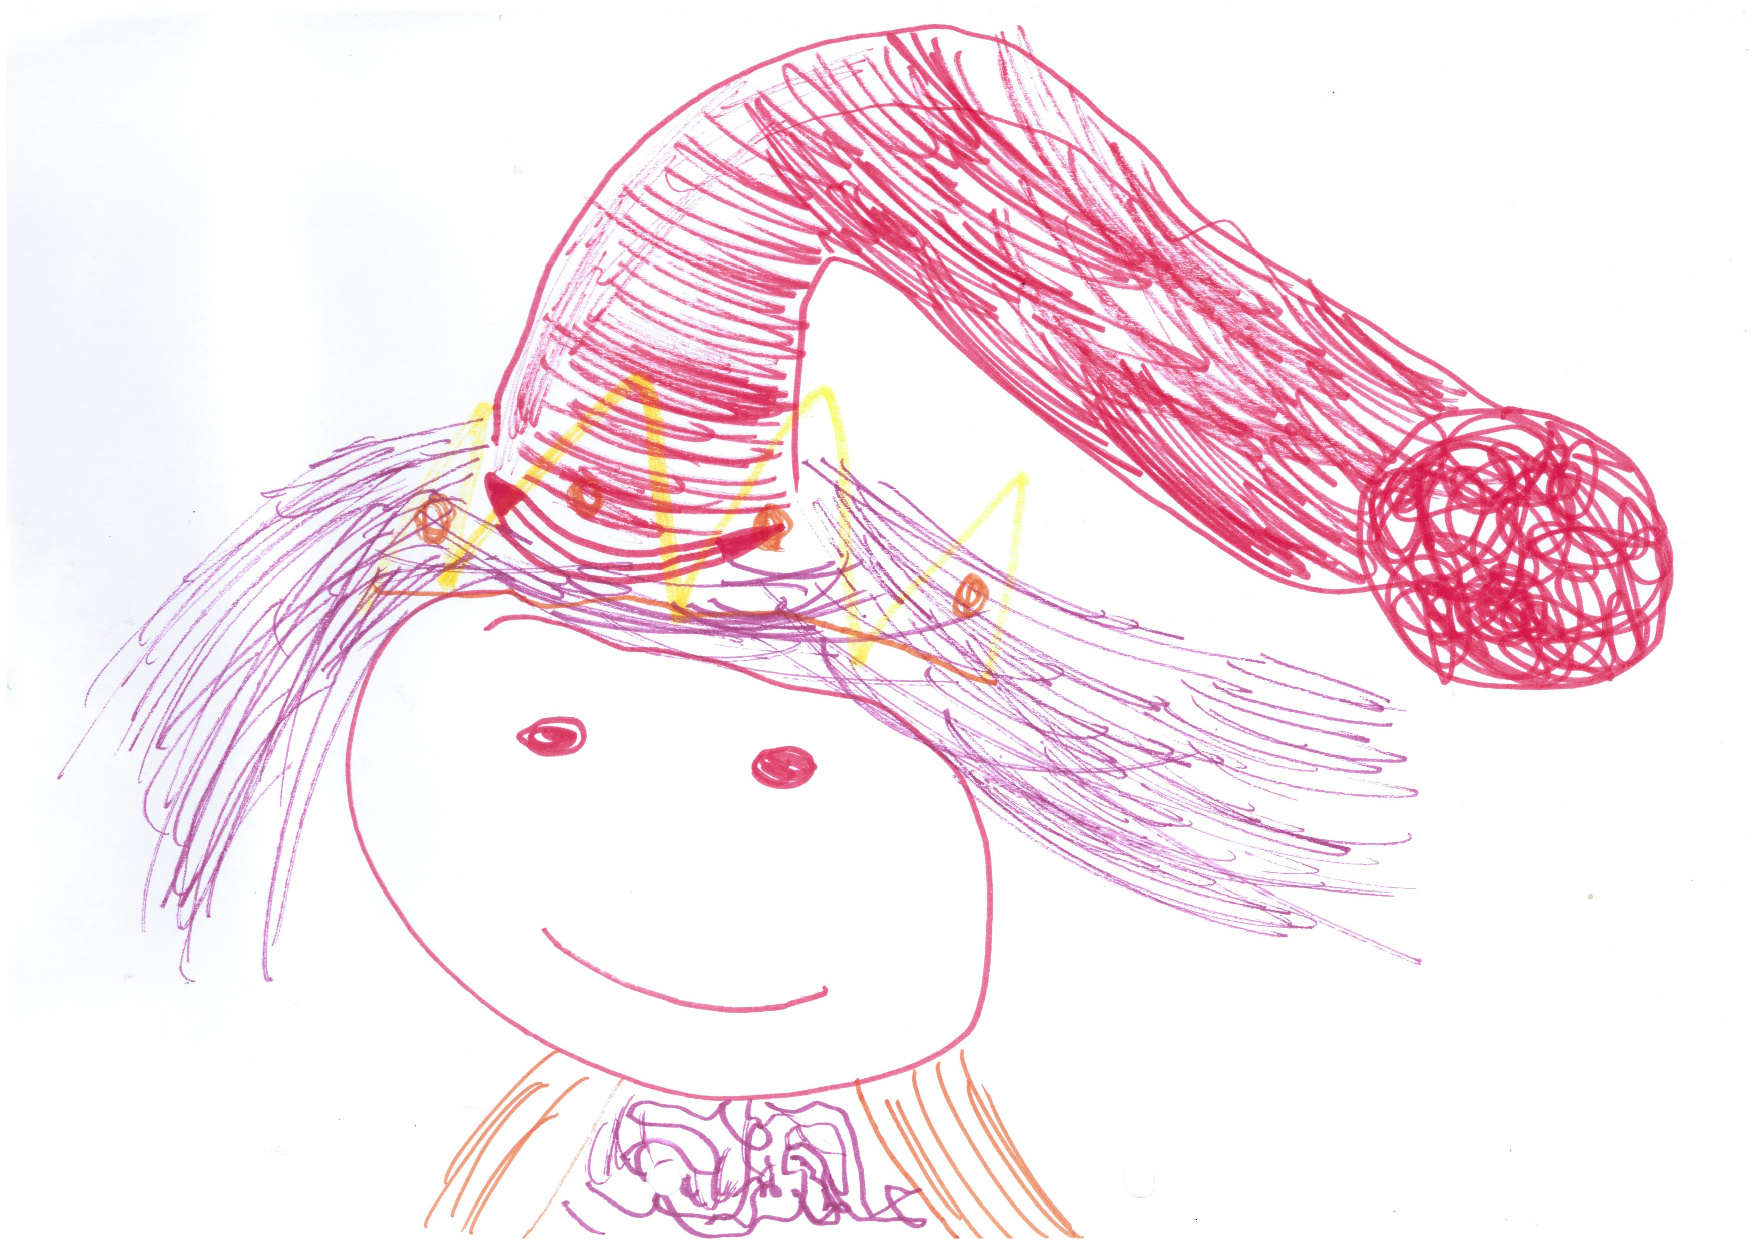
\includegraphics[width=\textwidth]{bilder/clown2.pdf}
\end{figure}

\enquote{Der grosse Clown kann fliegen!} ruft Louis immer wieder ganz aufgeregt.

Mama und Papa kommen ins Zimmer und wollen wissen, was hier los ist. Als sie verstanden haben, dass der Ballon durch das offene Fenster geflogen ist, schüttelt Papa den Kopf und Mama zieht die Augenbrauen hoch.

\enquote{Hast du nicht aufgepasst?} fragt Papa. \enquote{Na der ist weg.} ergänzt Mama, \enquote{Ich habe dir doch ein paar Mal erklärt, dass in dem Ballon Gas ist und der wegfliegt, wenn du nicht aufpasst.} Eltern treffen manchmal genau die Mitte zwischen einen Vorwurf machen und Trösten wollen. Na ja, dass der Ballon fliegen kann, hat Louis wirklich vergessen, denn er hatte ihn immer sehr fest im Arm gehalten. Aber trösten ist nicht nötig. Der Clown wird schon wissen, warum er weg geflogen ist. Und Louis weiss es auch. Jetzt kann Leika ihn nicht mehr beissen, jetzt ist er sicher.

Und weil Louis das weiss, macht es ihm auch gar nichts mehr, sich den Rest des Nachmittags ein bisschen um den Hund zu kümmern. Der ist ja jetzt der einzige, der wirklich enttäuscht ist.

 \hfill {\color{red}\decofourleft}
